\subsection{Motivation and Rationale}\label{subsec:motivation-and-rationale}

As mentioned, the motivation for trying these optimizers was to appropriately bound the strength of the 3 optimization techniques for CIFAR-10. 
This lays a strong groundwork for future additions to the algorithms and allows us to have a wide range of options in making these adjustments. 

DP-SGD is likely the most common optimization algorithm used in differentially private image classification. The motivation for using DP-SGD is simply to have a strong 
baseline for comparison. Most literature regarding differential privacy begins by using DP-SGD, so it would make sense as the first algorithm implemented and tested.

RMSProp and Adam can be viewed as successors to DP-SGD. Both introduce approaches that allow for adaptivity of the step size taken at each iteration of the algorithm. These algorithms
were first proposed to deal with the vanishing/exlpoding gradient phenomenon and have now been used frequently in the differentially private image classification literature. We felt that
implementing these algorithms would provide us with a strong bound on the performance benefits associated with changing optimizer, essentially treating optimizers as another hyperparameter
that we could tune.

\subsection{Description of Optimization Algorithm (Psuedocode)}\label{subsec:algorithm-description}

Below are pseudocodes for the DP-SGD, DP-RMSprop, and DP-Adam algorithms that we plan to privatize, adapted or referenced from~\cite{DBLP:journals/corr/abs-1807-06766}:

\begin{algorithm}[H]
    \caption{DP-SGD}
    \label{alg:sgd}
    \begin{algorithmic}[1]
        \State \textbf{Input:} A step size $\alpha$, initial starting point $\mathbf{x}_1 \in \mathbb{R}^d$,
        and access to a (possibly noisy) oracle for gradients of $f : \mathbb{R}^d \rightarrow \mathbb{R}$.
        \State Initialize: $\mathbf{v}_0 = \mathbf{0}$
        \For{$t = 1, 2, \dots$}
            \State Compute gradient $\mathbf{g}_t = \nabla f(\mathbf{x}_t)$
            \State Clip gradient $\mathbf{g}_t = \mathbf{g}_t / \max(1, \frac{\lVert \mathbf{g}_t \rVert_2}{C})$
            \State Add noise: $\hat{\mathbf{g}}_t = \mathbf{g}_t + \mathcal{N}(0, \sigma^2 C^2 I)$
            \State Descent: $\mathbf{x}_{t+1} = \mathbf{x}_t - \alpha \hat{\mathbf{g}}_t$
        \EndFor
    \end{algorithmic}
\end{algorithm}

\begin{algorithm}[H]
    \caption{DP-RMSProp}
    \label{alg:rmsprop}
    \begin{algorithmic}[1]
        \State \textbf{Input:} A constant vector $\mathbb{R}^d \ni \xi \mathbf{1}_d \geq 0$, parameter $\beta_2 \in [0, 1)$, step size $\alpha$, initial starting point $\mathbf{x}_1 \in \mathbb{R}^d$, and access to a (possibly noisy) oracle for gradients of $f : \mathbb{R}^d \rightarrow \mathbb{R}$.
        \State Initialize: $\mathbf{v}_0 = \mathbf{0}$
        \For{$t = 1, 2, \dots$}
            \State Compute gradient $\mathbf{g}_t = \nabla f(\mathbf{x}_t)$
            \State Clip gradient $\mathbf{g}_t = \mathbf{g}_t / \max(1, \frac{\lVert \mathbf{g}_t \rVert_2}{C})$
            \State Add noise: $\hat{\mathbf{g}}_t = \mathbf{g}_t + \mathcal{N}(0, \sigma^2 C^2 I)$
            \State Calculate moving average of squared gradient $\mathbf{v}_t = \beta_2 \mathbf{v}_{t-1} + (1 - \beta_2)(\hat{\mathbf{g}}_t^2 + \xi \mathbf{1}_d)$
            \State Descent: $\mathbf{x}_{t+1} = \mathbf{x}_t - \alpha \mathbf{V}_t^{-1/2} \hat{\mathbf{g}}_t$
        \EndFor
    \end{algorithmic}
\end{algorithm}

\begin{algorithm}[H]
    \caption{DP-Adam}
    \label{alg:adam}
    \begin{algorithmic}[1]
        \State \textbf{Input:} A constant vector $\mathbb{R}^d \ni \xi \mathbf{1}_d > 0$, parameters $\beta_1, \beta_2 \in [0, 1)$, a sequence of step sizes $\{\alpha_t\}_{t=1,2,\dots}$, initial starting point $\mathbf{x}_1 \in \mathbb{R}^d$, and oracle access to gradients of $f : \mathbb{R}^d \rightarrow \mathbb{R}$.
        \State Initialize: $\mathbf{m}_0 = \mathbf{0}$, $\mathbf{v}_0 = \mathbf{0}$
        \For{$t = 1, 2, \dots$}
            \State Compute gradient $\mathbf{g}_t = \nabla f(\mathbf{x}_t)$
            \State Clip gradient: $\mathbf{g}_t = \mathbf{g}_t / \max(1, \frac{\lVert \mathbf{g}_t \rVert_2}{C})$
            \State Add noise: $\hat{\mathbf{g}}_t = \mathbf{g}_t + \mathcal{N}(0, \sigma^2 C^2 I)$
            \State Calculate moving average of squared gradient: $\mathbf{v}_t = \beta_2 \mathbf{v}_{t-1} + (1 - \beta_2)(\hat{\mathbf{g}}_t^2 + \xi \mathbf{1}_d)$
            \State Calculate moving average of gradient: $\mathbf{m}_t = \beta_1 \mathbf{m}_{t-1} + (1 - \beta_1) \hat{\mathbf{g}}_t$
            \State Descent: $\mathbf{x}_{t+1} = \mathbf{x}_t - \alpha_t \frac{\mathbf{m}_t}{\sqrt{\mathbf{v}_t} + \epsilon}$
        \EndFor
    \end{algorithmic}
\end{algorithm}


\subsection{Proposed Modifications and Variations}\label{subsec:modification-and-variations}
Most of our current work has focused on implementing and testing the existing DP-SGD, DP-RMSProp, and DP-Adam optimization techniques. The main axes
of testing involved changing hyperparameters like epsilon, batch size, or noise level. This has allowed us to establish a base with 3 optimization techniques
that can each be used to test our proposed modifications and variations going forward.

Our next proposed approach will be privatizing Evolved Sign Momentum (Lion) optimizer. This optimization technique builds on variants of SGD and Adam and having 
differentially private implementations, of those, available should provide a good basis of comparison for our newly privatized version of Lion, DP-Lion. In the private world,
DP-SGD is still the most popular optimization technique, however in the non-private world, versions of Adam (AdamW) or Adafactor are the usual choices for training
a deep neural netwrok. \cite{chen2023symbolicdiscoveryoptimizationalgorithms} We feel that transitioning from the primary private optimizer to a newly privatized Lion optimizer
will be an interesting approach to examine.

To privatize Lion, we will need to add gaussian noise that is relative to the number of iterations, epsilon, and sensitivity. This will take a very similar form to the privatization
done for DP-SGD, DP-RMSProp, and DP-Adam. Next, we also plan to implement a clipping constant C, so as to properly bound the sensitivity associated with neighboring datasets. The following psuedocode
introduces our proposed adjustments to the Lion Optimizer from~\cite{chen2023symbolicdiscoveryoptimizationalgorithms}.


\begin{algorithm}
    \caption{DP-Lion}
    \label{alg:lion}
    \begin{algorithmic}[1]
        \State \textbf{Input:} A constant vector $\mathbb{R}^d \ni \xi \mathbf{1}_d > 0$, parameters $\beta_1, \beta_2 \in [0, 1)$, a sequence of step sizes $\{\alpha_t\}_{t=1,2,\dots}$, initial starting point $\mathbf{x}_1 \in \mathbb{R}^d$, and oracle access to gradients of $f : \mathbb{R}^d \to \mathbb{R}$.
        \State Initialize: $\mathbf{m}_0 = \mathbf{0}$
        \For{$t = 1, 2, \dots$}
            \State Compute gradient $\mathbf{g}_t = \nabla f(\mathbf{x}_t)$
            \State Clip gradient $\mathbf{g}_t = \mathbf{g}_t / \max(1, \frac{\lVert \mathbf{g}_t \rVert_2}{C})$
            \State Add noise: $\hat{\mathbf{g}}_t = \mathbf{g}_t + \mathcal{N}(0, \sigma^2 C^2 I)$
            \State Compute $c_{t} = \beta_1 m_{t-1} + (1 - \beta_1) \hat{\mathbf{g}}_t$
            \State Descent: $\mathbf{x}_t = \mathbf{x}_{t-1} - \alpha_t (\text{sign}(c_{t}) + \lambda \mathbf{x}_{t-1})$
            \State Calculate moving average of gradient $\mathbf{m}_t = \beta_2 \mathbf{m}_{t-1} + (1 - \beta_2) \hat{\mathbf{g}}_t$
        \EndFor
    \end{algorithmic}
\end{algorithm}


\subsection{Privacy Proof}\label{subsec:privacy-proof}

\subsection{Related Work: DP-SGD}\label{subsec:related-work}
Abadi et al. \cite{Abadi_2016_DeepLearningDifferentialPrivacy} introduced DP-SGD, which has become a foundational technique for
privacy-preserving model training. When specifically working on the CIFAR-10 dataset, this 2016 paper was able to achieve accuracies
of 65-75\% while keeping epsilon at or below 8. The biggest difference in their analysis and ours, is that they pretrain their convolutional
layers on CIFAR-100 before migrating to CIFAR-10, assuming that CIFAR-100 is a public dataset. Their results are seen below:
\begin{figure}[ht]
    \centering
    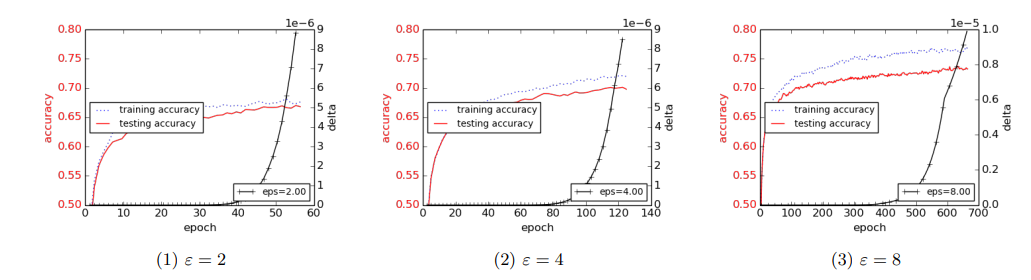
\includegraphics[width=\textwidth]{dp-sgd_results.PNG}
    \caption{DP-SGD Results on CIFAR-10 \cite{Abadi_2016_DeepLearningDifferentialPrivacy}}
    \label{fig:image_label}
\end{figure}

\subsection{Related Work: DP-RMSProp and DP-Adam}\label{subsec:related-work-RMSProp}
For comparison of DP-RMSProp and DP-Adam, we turn to the results from Zhou et al. (2020) \cite{zhou_2020_private_adaptive_algorithms}. They 
similarly 

\begin{figure}[ht]
    \centering
    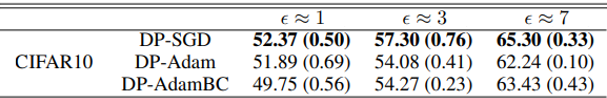
\includegraphics[width=\textwidth]{dp-adam-rms-results.PNG}
    \caption{DP-Adam Results on CIFAR-10 \cite{tang2023dpadambcdpadamactuallydpsgd}}
    \label{fig:image_label}
\end{figure}